\documentclass[a4paper]{exam}

\usepackage{amsmath, amssymb, amsthm, amsfonts}
\usepackage[utf8]{inputenc}
\usepackage{vntex}
\usepackage{tikz,tkz-tab}
\usepackage{graphicx}
\usepackage{float}


%Page setup
\usepackage[letterpaper, top = 1.0in, bottom = 1.0in, left = 1.0in, right = 1.0in, heightrounded]{geometry}

\headrule
\header{\textbf{Lời giải và bình luận: Trần Minh Đức}}{}{\textbf{Biên soạn: 7/3 - 8/3/2025}}

\begin{document}
	\begin{center}
		\fbox{\parbox{5.5in}{\centering
					\vspace{1mm}
					HCMUS - TOÁN RỜI RẠC (CNTT) - 13/11/2024\\
					\vspace{1mm}
					HỌC KÌ I - NĂM HỌC 2024 - 2025 - THỜI GIAN: 60 PHÚT\\
					\vspace{1mm}
				}
		}
	\end{center}
	
	\vspace*{2mm}
	
	\begin{questions}
		\question (\textbf{3.5 điểm} = 1đ + 1đ + 0.5đ + 1đ). \textbf{Cho các biến mệnh đề p, q, r, s và t.}
			\begin{itemize}
				\item Đặt $A = \left[((p \longrightarrow r) \land q) \longrightarrow (p \land q) \right]$ và $B = (\neg p \longrightarrow \neg q)$. Chứng minh $A \longleftrightarrow B$.\\
					\\Nếu p đúng thì chân trị của A ra sao? (Dùng B để giải thích ngắn gọn).\\
				\item Xét các suy luận sau:\\
					\[
					\begin{array}{c|c}
						\textbf{Suy luận bên trái} & \textbf{Suy luận bên phải}\\
						\hline
						\neg s \land t \quad (1) & r \lor t \quad (6)\\[1mm]
						p \lor q \quad (2) & \neg p \longrightarrow (q \land s) \quad (7)\\[1mm]
						q \longrightarrow (r \longrightarrow s) \quad (3) & p \land \neg t \quad (8)\\[1mm]
						t \longrightarrow q \quad (4) & r \longrightarrow \neg q \quad (9)\\[1mm]
						\hline
						\therefore p \quad (5) & \therefore \neg q \longrightarrow s \quad (10)
					\end{array}
					\]\\
					Hãy chứng minh suy luận bên trái là \textit{đúng} và giải thích tại sao suy luận bên phải là \textit{sai}.\\
				\item Cho $C = "\forall x \in \mathbb{R}, \exists y \in \mathbf{Q}, y = sin(3x)$ hay $y = cos(x)$. Viết mệnh đề phủ định $\neg C$ và xét chân trị của C.\\
			\end{itemize}
		\question (\textbf{3 điểm} = 1đ + 2đ)
			\begin{itemize}
				\item Cho $ A, B, C, D \subset E$. Chứng minh $\left[A \setminus (B \cup C) \right] \, \cup \, \left[(A \setminus B) \cap D \right] \, = \, \left[(A \setminus B) \setminus (C \cap \neg D)\right]$.\\
				\\Nếu $D = \emptyset$ thì hãy rút gọn $\left[(A \setminus B) \cap D \right]$ và $(C \cap \neg D)$.\\
				\item Cho $f: \mathbb{R} \longrightarrow \mathbb{R}$ có $f(x) = e^{-x} - 2e^{x} + 5, \forall x \in \mathbb{R}$, $g: \mathbb{R} \setminus \{0\} \longrightarrow \mathbb{R}$ có $g(x) = 2x^{2} - x^{-2} + 5, \forall x \in \mathbb{R} \setminus \{0\}$ và $h: \mathbb{R} \setminus \{0\} \longrightarrow \mathbb{R}$ thoả $f \circ g = h$.\\
				\\Chứng minh rằng $f$ là một song ánh và tìm biểu thức của ánh xạ ngược $f^{-1}$.\\
				\\Tìm biểu thức của $h$ (yêu cầu viết dưới dạng rút gọn).\\
 			\end{itemize}
 		\question (\textbf{3.5 điểm} = 1.5đ + 1đ + 1đ)
 			\begin{itemize}
 				\item Cho $S = {0, 1, 2,..., 8, 9, 10}$. Hỏi $S$ có bao nhiêu tập hợp con?\\
 				\\S có bao nhiêu tập hợp con T thoả $\|T\| = 6$, $minT = 1$ và $8 \leq maxT \leq 9$?\\
 				\item Xếp a, a, a, b, b, b, c, c, c, c thành một dãy ký tự tuỳ ý có 10 ký tự (chẳng hạn dãy \textit{cabcbaacbc},...). Hỏi có tất cả bao nhiêu dãy ký tự như vậy?\\
 				Nếu yêu cầu thêm ký tự đầu của dãy là a và ký tự cuối của dãy phải khác a thì ta có bao nhiêu dãy?\\
 				\item Khi khai triển biểu thức $(2x - 3y^{2} + 4z^{3} - 5t^{4})^{14} $ ta được bao nhiêu đơn thức khác nhau và hệ số đứng trước $x^{8}y^{4}z^{9}t^{4}$ là bao nhiêu?\\ 
 			\end{itemize}
	\end{questions}
	\hspace*{0pt}\hfill \textit{\textbf{HẾT}}
	
	\pagebreak
	
	\textit{\textbf{Câu 1:}}\\
	
	
	\textit{(a)} Nguyên tắc cơ bản nhất khi giải phương trình logic tương đương: \textbf{"Hoa sen nở"} - Giải quyết từng cụm mệnh đề từ trong ra ngoài và áp dụng các phép biển đổi thông dụng:\\
	
	Xét hai vế $A = \left[((p \longrightarrow r) \land q) \longrightarrow (p \land q) \right]$ và $B = (\neg p \longrightarrow \neg q)$
	
	\begin{equation*}
		\begin{aligned}
			A &\longleftrightarrow B \\
			\left[((p \longrightarrow r) \land q) \longrightarrow (p \land q) \right] 
			&\longleftrightarrow (\neg p \longrightarrow \neg q) \\ 
			((\neg p \lor r ) \land q) \longrightarrow (p \land q) 
			&\longleftrightarrow (\neg p \longrightarrow \neg q) \\ 
			\neg ((\neg p \lor r) \land q) \lor (p \land q) 
			&\longleftrightarrow (\neg p \longrightarrow \neg q) \\ 
			(p \land \neg r) \lor \neg q \lor (p \land q) 
			&\longleftrightarrow (\neg p \longrightarrow \neg q) \\ 
			(p \land \neg r) \lor (p \land q) \lor \neg q 
			&\longleftrightarrow (\neg p \longrightarrow \neg q) \\ 
			(p \land \neg r) \lor \underbrace{\left[(p \lor \neg q) \land (q \lor \neg q)\right]}_\textrm{Quy tắc phân phối}
			&\longleftrightarrow (\neg p \longrightarrow \neg q) \\ 
			\underbrace{(p \land \neg r) \lor p}_\textrm{Định lý hấp thu} \lor \neg q 
			&\longleftrightarrow (\neg p \longrightarrow \neg q) \\ 
			(p \lor \neg q) 
			&\longleftrightarrow (\neg p \longrightarrow \neg q) \\ 
			(\neg p \longrightarrow \neg q) 
			&\longleftrightarrow (\neg p \longrightarrow \neg q) 
		\end{aligned}
	\end{equation*}

	\hspace*{0pt}\hfill \textit{\textbf{Q.E.D}}\\
	
	Từ mệnh đề $A \longleftrightarrow B$ đã chứng minh như trên. Sử dụng vế B để biện luận chân trị của A:\\
	
	Nếu p đúng thì suy ra phủ định của p là sai $(\neg p = False)$, mặt khác ta lại có thêm hai trường hợp của q: Đúng và Sai (ở đây ta sẽ biểu hiện dưới dạng Boolean).
	
	\begin{itemize}
		\item \textbf{\textit{TH1: q = 1}} $ \longrightarrow (\neg p \longrightarrow \neg q) = 1$ 
		\item \textbf{\textit{TH2: q = 0}} $ \longrightarrow (\neg p \longrightarrow \neg q) = 1$ 
	\end{itemize}
	
	Tuy đầu vào khác nhau nhưng đều cho ra kết quả là 1 (True).\\
	
	\textit{(b)} Chứng minh suy luận bên trái và bên phải theo từng cặp.\\
	
	\textbf{Suy luận bên trái}:\\
	
	\[
	\begin{array}{c|c|c}
		\text{Tam đoạn luận (1)}                               & \text{Khẳng định (2)}           & \text{Tam đoạn luận rời (3)} \\ \hline
		q \longrightarrow (r \longrightarrow s)            & \neg r \lor (s \lor \neg t) & p \lor r                 \\
		t \longrightarrow q                                & \neg s \land t              & \neg r                   \\ \hline
		\therefore t \longrightarrow (r \longrightarrow s) & \therefore \neg r           & \therefore p                        \\
		\longleftrightarrow (\neg t \lor (\neg r \lor s))  &                             &
	\end{array}
	\]
	
	\hspace*{0pt}\hfill \textit{\textbf{Q.E.D}}\\
	
	\textbf{Suy luận bên phải}: Chứng minh bằng phản ví dụ\\
	
	Giả sử p = 1, t = 0. Vì t = 0 nên để mệnh đề (6) đúng thì r = 1 và từ r suy ra $\neg q = 1$. Phủ định của p = 0 thì $q \land s = 1$, nhưng vì tiền đề không đưa ra giả thuyết s nên ta không thể suy luận mệnh đề (10) $\longrightarrow$ \textit{Mâu thuẫn}\\
	
	\textit{(c)} $\neg C$ = "$\exists x \in \mathbb{R}, \forall y \in \mathbb{Q}, y = sin(3x)$ và $y = cos(x)$\\
	
	Xét chân trị của C hay hiểu cách khác là xác định nghiệm x sao cho giá trị y là số hữu tỉ.\\
	
	Với các nghiệm lượng giác x = \{$\frac{\pi}{2}$, 0\} thì đều cho ra số nguyên $\longrightarrow$ Loại.\\
	
	Với $x = \frac{\pi}{4}$ đều cho ra cả hai giá trị y = $\frac{\sqrt{2}}{2} \in \mathbb{Q} \longrightarrow$ Thoả.\\
	
	\textit{\textbf{Câu 2:}}\\
	
	\textit{(a)} Lưu ý hai tính chất quan trọng về phép toán tập hợp: $\overline{A \cap B} = \bar{A} \cup \bar{B}$ \textbf{(De Morgan)} và \textbf{hiệu của hai tập hợp} $(A \setminus B)$
	
	\begin{itemize}
		\item \textbf{Vế A: } $(A \setminus B) \cap (A \setminus C) = (A \cap \bar{B}) \cap (A \cap \bar{C} = A \cap B \cap \bar{C})$
		\item \textbf{Vế B: } $(A \setminus B) \cap D = A \cap \bar{B} \cap D$
	\end{itemize}
	
	Vế A $\cap$ Vế B = $(A \cap \bar{B}) \cap (\bar{C} \cup D) = (A \setminus B) \setminus (C \cap \bar{D})$\\
	
	Nếu $D = \emptyset \longrightarrow (A \setminus B) \cap D = \emptyset, \quad (C \cap \bar{D}) = C$\\
	
	\textit{(b)} Sơ lược ý tưởng chứng minh:
	
	\begin{itemize}
		\item Một hàm số được xem là song ánh khi và chỉ khi nó vừa là đơn ánh, vừa là toàn ánh.
		\item Đơn ánh (One-to-one function): với mỗi nghiệm x sẽ cho ra một giá trị y khác nhau.
		\item Toàn ánh (Surjective function): $\{\forall x \in \mathbb{R} | y = f(x) \}$ 
	\end{itemize}
	
	Đối vối một số trường hợp hàm số luỹ thừa, bậc cao không thể áp dụng phương pháp biến đổi thông thường, ta có thể nghĩ đến việc áp dụng phương pháp giải tích (xét sự biến thiên của hàm số $f'(x)$). Dưới đây là một số trường hợp cần lưu ý:
	
	\begin{itemize}
		\item $f'(x) > 0, f'(x) < 0$ tức hàm số đồng biến / nghịch biến trên mọi khoảng xác định $\longrightarrow$ $f(x)$ là một đơn ánh.
		\item Nhưng nếu $f'(x) = 0$ tại một vài điểm cực trị (xem như nó là tập hợp A gồm các điểm cực trị), khảo sát đạo hàm bậc 2 (điểm lồi trên, lồi dưới). Nếu $f''(x) = 0$ tồn tại ở vài điểm trong tập A, tiếp tục kiểm tra đạo hàm bậc 3 trong tập B $(B \subset A)$. Nếu $f'''(x) \neq 0$ trong tất cả những điểm thuộc tập B $\longrightarrow$ Hàm số là một đơn ánh.
		
	\end{itemize}
	
	Xét $f(x) = e^{-x} - 2e^{x} + 5, \forall x \in \mathbb{R} \iff f'(x) = -e^{-x} - 2e^{x} < 0$ (Nghịch biến)\\
	
	Kiểm tra giới hạn tại các điểm cận trên, cận dưới \textbf{(Chứng minh cho tính chất toàn ánh)}:\\ 
	$$ \lim_{x \to \infty} f(x) = \lim_{x \to \infty} e^{-x} - 2e^{x} + 5 = -\infty $$
	$$ \lim_{x \to -\infty} f(x) = \lim_{x \to \infty} e^{-x} - 2e^{x} + 5 = \infty $$\\
	
	Lập bảng biến thiên của hàm số $f(x)$:\\
	\begin{center}
		
		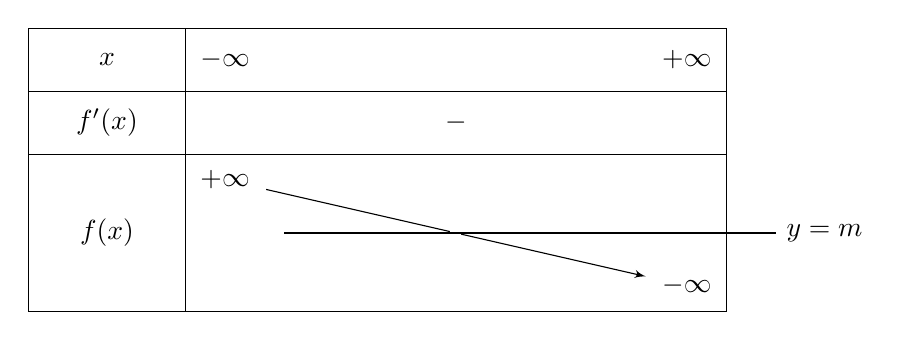
\begin{tikzpicture}
			\tkzTabInit
			[lgt=2,espcl=0.0085\linewidth] % tùy chọn
			{$x$/.8, $f’(x)$/.8, $f(x)$/2} % cột đầu tiên
			{$-\infty$,$$,$+\infty$} % hàng 1 cột 2
			\tkzTabLine{,,-,,} % hàng 2 cột 2
			\tkzTabVar{+/ $+\infty$ , R/ , -/ $-\infty$} % hàng 3 cột 2 (2 điểm đầu)
			\tkzTabIma{1}{3}{2}{$$} % hàng 3 cột 2 (điểm giữa
	 	\draw[black, thick] (3.25,-2.6) -- (9.5,-2.6) node[right, black] {$y = m$};
		\end{tikzpicture}
		
	\end{center}
	
	\underline{Nhận xét}: Với mọi giá trị m tại mỗi điểm x đều luôn tồn tại duy nhất một nghiệm thực khác nhau. 
	$\Longrightarrow f(x)$ vừa là toàn ánh, đơn ánh (Song ánh).
	
	\hspace*{0pt}\hfill \textit{\textbf{Q.E.D}}\\
	
	Vì f là một song ánh nên ta biết rằng với mỗi nghiệm phương trình luôn tồn ánh xạ ngược $f^{-1}$.\\
	
	Đặt $y = e^{-x} - 2e^{x} + 5$ 
	\begin{equation}
		\label{eq:important}
		\Longleftrightarrow y = \frac{1 - 2e^{2x} + 5e^{x}}{e^{x}} \Longleftrightarrow ye^{x} = 1 - 2e^{2x} + 5e^{x} \Longleftrightarrow -2e^{2x} + (5 - y)e^{x} + 1 = 0
	\end{equation}
	
	Giải phương trình bằng công thức nghiệm bậc 2:
	\begin{align*}
		\eqref{eq:important} \Longrightarrow \Delta = b^{2} - 4ac = (5 - y)^{2} + 8 > 0
	\end{align*}
	
	$$
	\Longrightarrow \begin{cases}
		x_1 = \frac{-b + \sqrt{\Delta}}{2a}\\
		x_2 = \frac{-b - \sqrt{\Delta}}{2a}\\
	\end{cases} 
	\Longleftrightarrow \begin{cases}
			x_1 = \frac{-b + \sqrt{(5 - y)^{2} + 8}}{-4}\\
			x_2 = \frac{y - 5 - \sqrt{(5 - y)^{2} + 8}}{-4}\\
	\end{cases}
	\Longleftrightarrow \begin{cases}
			x_1 = \frac{y - 5 + \sqrt{(5 - y)^{2} + 8}}{-4}\\
			x_2 = \frac{5 - y + \sqrt{(5 - y)^{2} + 8}}{4}\\
	\end{cases}
	$$	
	
	Dễ thấy nghiệm $x_{1} < 0$ nên ta chỉ nhận nghiệm $x_{2}$\\
	
	$$ \Longrightarrow e^{x} = \frac{5 - y + \sqrt{(5 - y)^{2} + 8}}{4} \\
	\Longrightarrow x = \ln \left( \frac{5 - y + \sqrt{(5 - y)^{2} + 8}}{4} \right)= f^{-1}(y)$$\\
	
	Tiếp theo, đề bài cho biết dữ kiện của hàm hợp (Composite Function) $f \circ h = g \longrightarrow f(h(x)) = g(x)$\\
	
	Muốn truy ngược nguồn gốc của hàm h(x) - trớ trêu thay ở dưới dạng hàm hợp của f(x), ta áp dụng tính chất của ánh xạ ngược:
	
	\begin{figure}[H]
		\centering
		\includegraphics[totalheight=2.75cm]{finvCircf.png}  % File name only
		\label{fig:inverse_prop}
	\end{figure}
	
	$$f \circ h = g \Longleftrightarrow f^{-1} \circ f \circ h = f^{-1} \circ g \Longleftrightarrow h = f^{-1} \circ g = \ln \left( \frac{-2x^{2} + x^{-2} + \sqrt{(x^{-2} - 2x^2)^2 + 8}}{4} \right) $$	
	
	$$ = \ln \left( \frac{-2x^2 + x^{-2} + 2x^{2} + x^{-2}}{4} \right) = \ln \left( \frac{-x^{2}}{2} \right)$$.
	
	\textit{\textbf{Câu 3:}}\\
	
	\textit{(a)} $S = \{ 0, 1, 2, ..., 8, 9, 10\} \Longrightarrow$ Số tập hợp con là $2^{11} = 2048$\\
	
	Tập hợp con thoả $\|T\| = 6$, $minT = 1$ và $8 \leq maxT \leq 9$\\
	
	Diễn giải từng điều kiện ràng buộc: 
	
	\begin{itemize}
		\item Giới hạn của một tập số nguyên có thể có là 6
		\item Giá trị nhỏ nhất của một giá trị có trong tập T là 1 và giá trị lớn nhất trong tập có thể là 8 hoặc 9
	\end{itemize}
	
	Vì ta đã biết giá trị nhỏ nhất mặc định là 1 nên chỉ cần xét hai trường hợp khi $maxT = 8$ và $maxT = 9$:\\

		\textbf{TH1}: $maxT = 8 \longrightarrow S_{1} = \{2; 3; 4; 5; 6; 7\} \Longrightarrow 
			\begin{array}{|c|c|c|c|c|c|}
				1 & \_ & \_ & \_ & \_ & 8
			\end{array} \Longrightarrow \binom{6}{4} = \frac{6!}{4! \cdot 2!} = 15$ (tập)\\
			
		\textbf{TH2}: $maxT = 9 \longrightarrow S_{2} = \{2; 3; 4; 5; 6; 7; 8\} \Longrightarrow 
			\begin{array}{|c|c|c|c|c|c|}
				1 & \_ & \_ & \_ & \_ & 9
			\end{array} \Longrightarrow \binom{7}{4} = \frac{7!}{4! \cdot 3!} = 30$ (tập)\\
	
	Vậy tổng số tập hợp con T thoả mãn những điều kiện ràng buộc là $15 + 35 = 50$.\\
	
	\textit{(b)} Xếp các chữ cái tuỳ ý thành một dãy có 10 ký tự gồm 3a, 3b và 4c\\
	
	$\Longrightarrow \binom{10}{3,3,4} = \frac{10!}{3! \cdot 3! \cdot 4!} = 4200$ (cách)\\
	
	Mặt khác đề bài thêm yêu cầu ký tự đầu của dãy là a và ký tự cuối phải khác a. Không xét với trường hợp a đứng đầu mà chỉ xét 2 trường hợp b hoặc c nằm cuối, lý do bởi nếu ta thêm dữ kiện trước dẫn đến sự lặp lại của những trường hợp ta đã bỏ qua.\\
	
	\textbf{TH1}: Vị trí cuối là chữ cái "b" $\Longrightarrow \binom{8}{2,2,4} = \frac{68!}{2! \cdot 2! \cdot 4!} = 420$ (cách)
	
	\begin{center}
		\[
		\begin{array}{|c|c|c|c|c|c|c|c|c|c|c|}
			a & \multicolumn{8}{c|}{\underbrace{\quad \_ \quad \_ \quad \_ \quad \_ \quad \_ \quad \_ \quad \_ \quad \_ \quad}_{\text{2a, 2b, 4c}}} & b
		\end{array}
		\]
	\end{center}
	
	\textbf{TH2}: Vị trí cuối là chữ cái "c" $\Longrightarrow \binom{8}{2,3,3} = \frac{68!}{2! \cdot 3! \cdot 3!} = 560$ (cách)
	
	\begin{center}
		\[
		\begin{array}{|c|c|c|c|c|c|c|c|c|c|c|}
			a & \multicolumn{8}{c|}{\underbrace{\quad \_ \quad \_ \quad \_ \quad \_ \quad \_ \quad \_ \quad \_ \quad \_ \quad}_{\text{2a, 3b, 3c}}} & c
		\end{array}
		\]
	\end{center}

	Như vậy tổng tất cả khả năng lập thành 1 dãy ký tự thoả mãn những điều kiện ràng buộc là $420 + 560 = 980$ (cách)\\
	
	\textit{(c)} Đối với vấn đề đầu tiên: Có bao nhiêu số hạng được khai triển với 4 biến số trên bậc thứ 14. Quy về thành bài toán như sau:\\
	
	\textbf{"Có bao nhiêu số nghiệm nguyên không âm của phương trình thoả $x + y + z + t = 14$ ?"}\\
	
	Giải thích cho điều này, ngoài các đơn thức riêng lẻ sau khi bung ra $x^{14}, y^{14}, z^{6},...$ thì còn có đa thức nối liền $x^{12}yzt, xy^{6}zt, xyzt^{7},...$ và nếu tinh ý sẽ phát hiện các biến số ấy luôn có những cụm lặp, được sắp xếp tuỳ ý. Do đó, từ hệ quả của tổ hợp lặp:\\
	
	Số nghiệm nguyên không âm $(x_{1}, x_{2}, ..., x_{n}) (x_{i} \in \mathbb{Z}, x_{i} \geq 0)$  
	
	$$x_{1} + x_{2} + ... + x_{n} = r$$
	
	là 
	\[
	K_n^r = C_{r+n-1}^r.
	\]
	
	Áp dụng công thức như trên ta được: $K_{14}^4 = C_{17}^{14} = 680 $ (nghiệm). Vậy có 680 đơn thức được khai triển từ hàm đa thức.\\
	
	Cuối cùng, giải quyết vế sau bằng ý niệm sử dụng \textbf{\textit{nhị thức Newton}} để tìm hệ số $x^{8}y^{4}z^{9}t^{4}$ không mấy khả thi ít nhất về mặt số lượng biến số hiện diện và độ phức tạp khi triển khai từ bậc thứ 3 trở đi. Sâu xa hơn về mặt ý nghĩa thâm thuý trong vấn đề tối ưu thuật toán và tiềm ẩn phát sinh, chẳng hạn như điểm yên ngựa (Saddle point - một điểm trên bề mặt đồ thị hàm số mà tại đó đạo hàm bằng không nhưng không tồn tại miền giá trị lớn nhất - nhỏ nhất cục bộ).\\
	
	Thay vào đó, ta có thể nghĩ đến việc áp dụng \textbf{\textit{định lý đa thức (Multinomial Theorem)}}:\\
	
	Cho $x_{1}, x_{2}, ..., x_{m}$ là các biến và n là số nguyên dương. Khi đó
	
	\[
		(x_{1} + x_{2} + ... + x_{m})^{n} = \sum_{k_{1} + k_{2} + ... + k_{m} = n} \frac{n!}{k_{1}! \cdot k_{2}! ... k_{m}!} x_{1}^{k_{1}} \cdot x_{2}^{k_{2}} ... x_{m}^{k_{m}}
	\]\\
	
	\textit{Lưu ý: Các biến số trong hàm đa thức $(2x - 3y^{2} + 4z^{3} - 5t^{4})^{14} $ không phải bậc nhất nên ta phải truy ngược các bội số gốc $k_{1}, k_{2}, ..., k_{m}$}
	
	\begin{itemize}
		\item $x_{1}^{k_{1}} = (2x)^{k_{1}} = 2^{k_{1}} x^{k_{1}} \Longrightarrow x^{k_{1}} = x^{8} \Longleftrightarrow \boxed{k_{1} = 8}$
		\item $x_{2}^{k_{2}} = (-3y^{2})^{k_{2}} = (-3)^{k_{2}} y^{2k_{2}} \Longleftrightarrow y^{2k_{2}} = y^{4} \Longleftrightarrow \boxed{k_{2} = 2}$
		\item $x_{3}^{k_{3}} = (4z^{3})^{k_{3}} = 4^{k_{3}} z^{3k_{3}} \Longleftrightarrow z^{3k_{3}} = z^{9} \Longleftrightarrow \boxed{k_{3} = 3}$
		\item $x_{4}^{k_{4}} = (-5t^{4})^{k_{4}} = (-5)^{k_{4}} t^{4k_{4}} \Longleftrightarrow t^{4k_{4}} = t^{4} \Longleftrightarrow \boxed{k_{4} = 1}$
	\end{itemize}
	
	Áp dụng định lý như trên, số hạng chứa $x^{8}y^{4}z^{9}t^{4}$ là:
		
	\[
		\frac{14!}{8! \cdot 2! \cdot 3! \cdot 1!} (2x)^{8} \cdot (-3y^{2})^{2} \cdot (4z^{3})^{3} \cdot (-5t^{4}) = \frac{14!}{8! \cdot 2! \cdot 3! \cdot 1!} \cdot 2^{8} \cdot 9 \cdot 64 \cdot (-5) \cdot (x^{8}y^{4}z^{9}t^{4}) =  -132843110400x^{8}y^{4}z^{9}t^{4}
	\]
	
	Vậy hệ số của $x^{8}y^{4}z^{9}t^{4}$ là -132843110400.\\
	
	\hspace*{0pt}\hfill \textit{\textbf{HẾT}}
	
	
	
	
\end{document}